\documentclass{article}
\usepackage{amsmath}
\usepackage{amssymb}
\usepackage{graphicx}
\usepackage[margin=1in]{geometry}
\usepackage{hyperref}
\usepackage{caption}
\usepackage{float}
\usepackage{tikz}
\graphicspath{{images/}}
\hypersetup{
  colorlinks=true,
  urlcolor=blue,
}
\begin{document}

\title{An Original Puzzle}
\author{Aresh Pourkavoos}
\maketitle

I came up with this math competition-style puzzle recently.
Consider a $5 \times 5$ grid whose cells may be either white or black.
All cells are initially white.
We may select a rectangle within this grid
and invert the colors of the cells within the rectangle.
For example, the result of two such operations in order are below:

\begin{center}
  \scalebox{0.5}{
    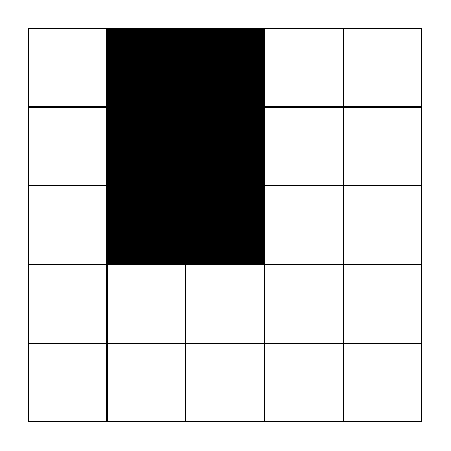
\begin{tikzpicture}[every node/.style={minimum size=1cm-\pgflinewidth, outer sep=0pt}]
      \draw[shift={(-0.5,-0.5)},step=1cm,color=black] (0,0) grid (5,5);
      \node[fill=black] at (1,2) {};
      \node[fill=black] at (2,2) {};
      \node[fill=black] at (1,3) {};
      \node[fill=black] at (2,3) {};
      \node[fill=black] at (1,4) {};
      \node[fill=black] at (2,4) {};
    \end{tikzpicture}
  }
  \scalebox{0.5}{
    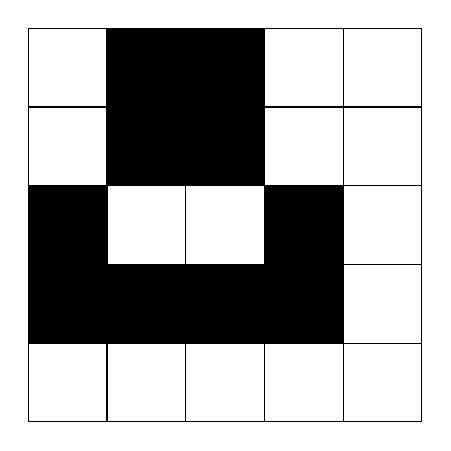
\begin{tikzpicture}[every node/.style={minimum size=1cm-\pgflinewidth, outer sep=0pt}]
      \draw[shift={(-0.5,-0.5)},step=1cm,color=black] (0,0) grid (5,5);
      \node[fill=black] at (0,1) {};
      \node[fill=black] at (1,1) {};
      \node[fill=black] at (2,1) {};
      \node[fill=black] at (3,1) {};
      \node[fill=black] at (0,2) {};
      \node[fill=black] at (3,2) {};
      \node[fill=black] at (1,3) {};
      \node[fill=black] at (2,3) {};
      \node[fill=black] at (1,4) {};
      \node[fill=black] at (2,4) {};
    \end{tikzpicture}
  }
\end{center}
The first rectangle inverted is 3 cells tall and 2 cells wide,
and the second is $2 \times 4$.
The puzzle is:
How many distinct ways are there
to create the pattern below
using exactly four of these operations,
starting from a fully white board?

\begin{center}
  \scalebox{0.5}{
    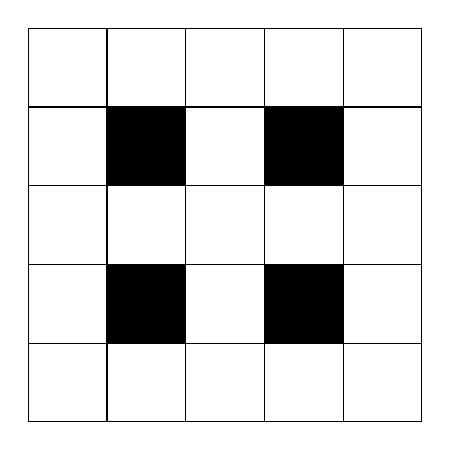
\begin{tikzpicture}[every node/.style={minimum size=1cm-\pgflinewidth, outer sep=0pt}]
      \draw[shift={(-0.5,-0.5)},step=1cm,color=black] (0,0) grid (5,5);
      \node[fill=black] at (1,1) {};
      \node[fill=black] at (1,3) {};
      \node[fill=black] at (3,1) {};
      \node[fill=black] at (3,3) {};
    \end{tikzpicture}
  }
\end{center}

For example, these four rectangles constitute one way:
\begin{center}
  \scalebox{0.5}{
    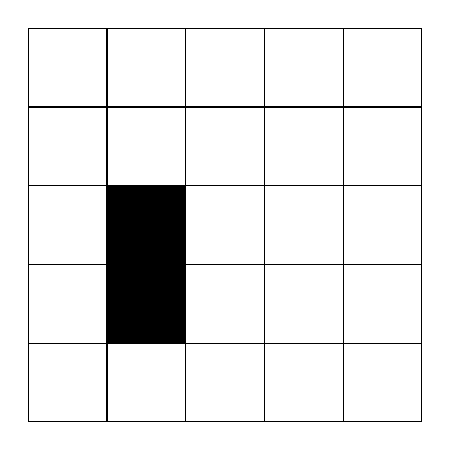
\begin{tikzpicture}[every node/.style={minimum size=1cm-\pgflinewidth, outer sep=0pt}]
      \draw[shift={(-0.5,-0.5)},step=1cm,color=black] (0,0) grid (5,5);
      \node[fill=black] at (1,1) {};
      \node[fill=black] at (1,2) {};
    \end{tikzpicture}
  }
  \scalebox{0.5}{
    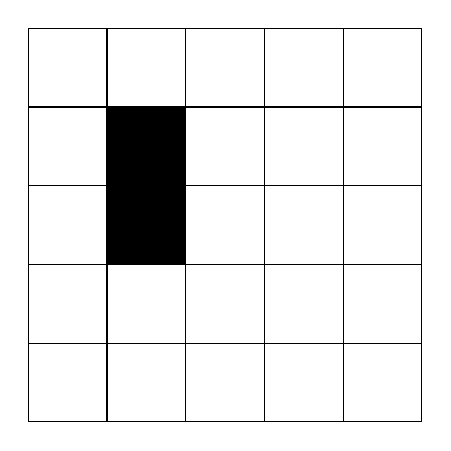
\begin{tikzpicture}[every node/.style={minimum size=1cm-\pgflinewidth, outer sep=0pt}]
      \draw[shift={(-0.5,-0.5)},step=1cm,color=black] (0,0) grid (5,5);
      \node[fill=black] at (1,2) {};
      \node[fill=black] at (1,3) {};
    \end{tikzpicture}
  }
  \scalebox{0.5}{
    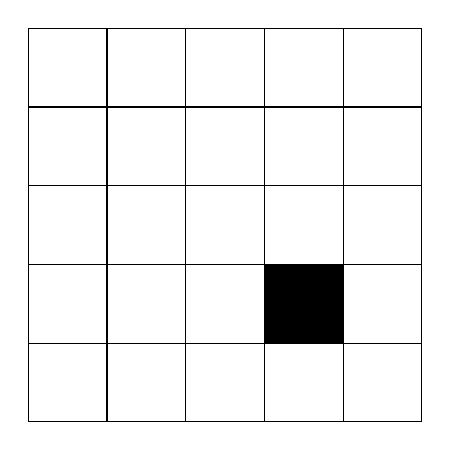
\begin{tikzpicture}[every node/.style={minimum size=1cm-\pgflinewidth, outer sep=0pt}]
      \draw[shift={(-0.5,-0.5)},step=1cm,color=black] (0,0) grid (5,5);
      \node[fill=black] at (3,1) {};
    \end{tikzpicture}
  }
  \scalebox{0.5}{
    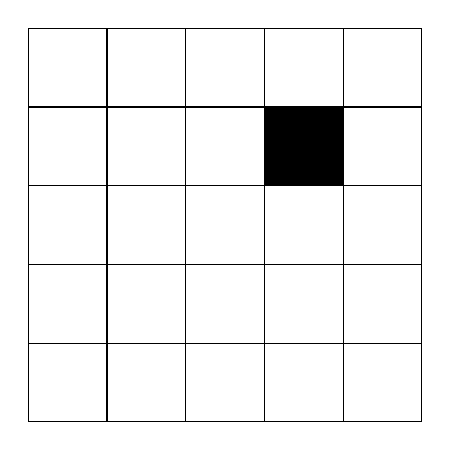
\begin{tikzpicture}[every node/.style={minimum size=1cm-\pgflinewidth, outer sep=0pt}]
      \draw[shift={(-0.5,-0.5)},step=1cm,color=black] (0,0) grid (5,5);
      \node[fill=black] at (3,3) {};
    \end{tikzpicture}
  }
\end{center}
The two rectangles on the left overlap in one square, which ``cancels out''
and becomes white in the final result.

\end{document}
